\chapter{Results}

\section{Responses to Temperature Anomalies}

\definecolor{codegreen}{rgb}{0,0.6,0}
\definecolor{codegray}{rgb}{0.5,0.5,0.5}
\definecolor{codepurple}{rgb}{0.58,0,0.82}
\definecolor{backcolour}{rgb}{0.95,0.95,0.92}

\lstdefinestyle{mystyle}{
    backgroundcolor=\color{backcolour},   
    commentstyle=\color{codegreen},
    keywordstyle=\color{magenta},
    numberstyle=\tiny\color{codegray},
    stringstyle=\color{codepurple},
    basicstyle=\footnotesize,
    breakatwhitespace=false,         
    breaklines=true,                 
    captionpos=b,                    
    keepspaces=true,                 
    numbers=left,                    
    numbersep=5pt,                  
    showspaces=false,                
    showstringspaces=false,
    showtabs=false,                  
    tabsize=2
}

\lstset{style=mystyle}

As a reminder, our hypothesis for the temperature anomalies was that the body mass of the species largely determined the number of individuals seen at the feeders during periods of cold temperatures. The larger massed birds have an easier time retaining heat and thus would not be required to visit the bird feeders as often. The smaller birds have to eat more food in order to make up for the calories that are lost trying to stay warm during the colder days. We ignored the evolutionary and behavior differences among the species and instead focused on the thermoregulation requirements of the birds in regards to the body mass. Thus the body mass values of the species play a key role in the results and further analysis. 

We expected to see that as the body mass of the bird species increases so does the slope estimate of the model, as the slope becomes less negative. The sign of the slope estimate is key. With the t value, we expected the opposite relationship, as the body mass increases the t value decreases in magnitude, as this indicates there is less of an effect of temperature variation.


% Please add the following required packages to your document preamble:
% \usepackage{longtable}
% Note: It may be necessary to compile the document several times to get a multi-page table to line up properly
\begin{longtable}[c]{|l|l|l|l|l|}
\caption{Linear-mixed Models: log(Nseen) as a function of temperature anomalies. Slope Estimates and t-values for all of the bird species for the temperature anomalies analysis. The rows are in increasing order by body mass of the species.}
\label{my-label}\\
\hline
Bird Species              & Body Mass (grams) & Slope Estimate & t-value & Sig.     \\ \hline
\endhead
%
Brown Creeper             & 7.5               & -0.0006486     & -1.215  & not sig. \\ \hline
Chestnut-backed Chickadee & 9.5               & -0.00862       & -4.276  & sig.     \\ \hline
Mountain Chickadee        & 11                & -0.002494      & -2.003  & sig.     \\ \hline
Black-capped Chickadee    & 11.5              & -0.001069      & -0.624  & not sig. \\ \hline
Chipping Sparrow          & 13.5              & 0.001731       & 1.274   & not sig. \\ \hline
Pine Siskin               & 15                & -0.008119      & -2.653  & sig.     \\ \hline
American Goldenfinch      & 15.5              & -0.006899      & -3.334  & sig.     \\ \hline
Common Redpoll            & 15.5              & -0.003651      & -1.336  & not sig. \\ \hline
Tufted Titmouse           & 22                & -0.004384      & -4.018  & sig.     \\ \hline
Dark-eyed Junco           & 24                & -0.028332      & -15.38  & sig.     \\ \hline
Downy Woodpecker          & 24.5              & -0.0032084     & -3.35   & sig.     \\ \hline
White-throated Sparrow    & 27                & -0.021324      & -13.44  & sig.     \\ \hline
Northern Cardinal         & 45                & -0.017232      & -8.11   & sig.     \\ \hline
Northern Mockingbird      & 51.5              & 0.0033151      & 6.43    & sig.     \\ \hline
Pine Grosbeak             & 56.4              & -0.02334       & -2.929  & sig.     \\ \hline
Evening Grosbeak          & 63.5              & 0.01041        & 2.001   & sig.     \\ \hline
Hairy Woodpecker          & 67.5              & -0.0010992     & -1.475  & not sig. \\ \hline
Red-bellied Woodpecker    & 73.5              & -0.0008638     & -1.402  & not sig. \\ \hline
European Starling         & 78                & -0.015726      & -7.305  & sig.     \\ \hline
Blue Jay                  & 85                & -0.015082      & -5.624  & sig.     \\ \hline
Common Grackle            & 108               & 0.015218       & 5.003   & sig.     \\ \hline
Mourning Dove             & 121               & -0.016746      & -6.754  & sig.     \\ \hline
Black-billed Magpie       & 177.5             & -0.003586      & -2.368  & sig.     \\ \hline
All species               & NA                & -7.38E-03      & -15.31  & sig.     \\ \hline
\end{longtable}

Table 4.1 presents the slope estimates for the linear-models constructed with temperature deviations as the independent variable and the natural log of number seen as the dependent variable. The t values are also presented in the column labeled t-value. The majority of the observations are considered significant enough to draw insights from, with only 6 of the 23 observations having absolute t values lower than 2. 

In order to ensure the validity of our analysis, all non significant rows were ignored in the constructed data set. These ignored tuples all had an absolute t value of less than 2, indicating that the relationships were not strong enough to support insights. All of the remaining tuples contain statistically valid data, which can be confidently analyzed. The scatter plot of the slope estimates and body mass values from Table 4.1 is presented in Figure 4.1.

\begin{figure}[h]
\centering
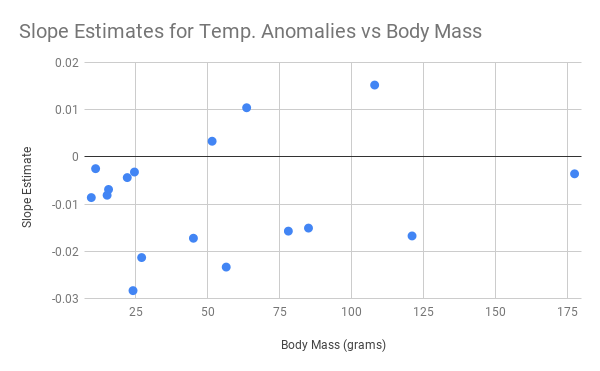
\includegraphics[width=1.0\textwidth]{figures/tempScaledvsBodyMass.png}
\caption{The plot shows the relationship between the slope estimates for the linear-mixed models with temperature anomalies being the independent variable.}
\end{figure}

From the scatter plot in Figure 4.1 it becomes clear that many of the bird species tended to visit the bird feeders more often as the temperature fell below average. Only 3 bird species, all of them with mid range body mass, have positive slopes. Interestingly, the Evening Grosbeak is one of those species. This stands out because this species is also suffering range-wide decline in population at the feeders~\cite{bonter2008winter}. The largest of the bird species analyzed, with a body mass of 177.5 grams, has a negative slope. Thus in a larger sense our hypothesis was correct, bird species in general are more abundant at the feeders during especially at colder temperatures.  

However, there is yet no support from this study that body mass in fact determines the number of individuals seen. This is made clear by the scatter plot. The smallest massed species, those with body masses from 9.5 grams to 24.5 grams, have negative slope estimate values that are almost equivalent to the negative slope estimates of the largest species, with a body mass of 177.5 grams.

For a visual representation of the data points being analyzed in these models refer to Figures 4.2 and 4.3. These are for the species American Goldfinch and Evening Grosbeak, respectively. The figures plot the relationship between the natural log of Nseen and temperature anomalies. There are far too many data points in the plots to observe any trends by eye, thus the use of the models throughout this analysis. However, it is still worthwhile to scan the data point distributions that are present.

\begin{figure}[h]
\centering
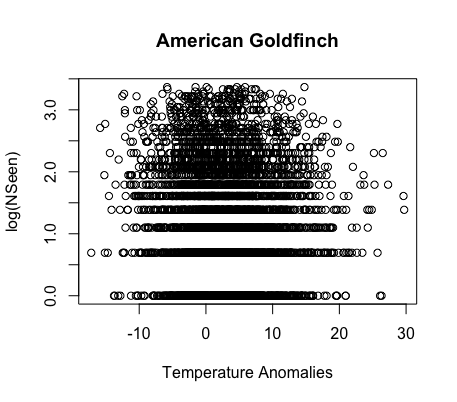
\includegraphics[width=10cm]{figures/amegfi_plot.png}
\caption{Data points for the American Goldfinch.}
\end{figure}

\begin{figure}[h]
\centering
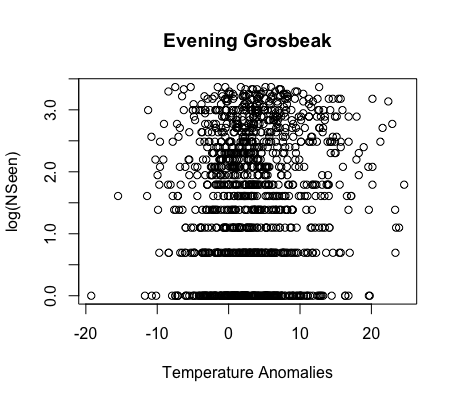
\includegraphics[width=10cm]{figures/evegros_plot.png}
\caption{Data points for the Evening Grosbeak.}
\end{figure}

Another simple linear model was constructed with just the body mass and slope estimate data. The code for constructing this model using R programming language is presented below. The independent variable for this model is the natural log of the body mass and the dependent variable is the slope estimate for the temperature anomalies. The natural log is used again in order to make the left skew less prominent. This allows for a more reliable linear model.  

\begin{lstlisting}[language=R]
model <- lm(tempAnomaliesSlopeEstimates ~ log(bodyMass))
\end{lstlisting}

According to our hypothesis there should be a positive relationship or slope for this simple model. However, the relationship presented in the linear model above is not significant enough to warrant insight. It has a t value of 0.326, which is far below 2, indicating there is a very weak effect of body mass on the slope estimates. This is further evidence that body mass does not determine the frequency of feeder visits due to cold temperatures. 

The second value of importance is the t value for the species linear-mixed models. As a reminder the magnitude of the t-value determined the strength of the effect of the temperature anomalies on the abundance at the feeders. Table 4.1 also presents the body mass of the species and the t-values. The negative and positive signs on the values are only related to the slope intercept sign, and serve no purpose in assessing the strength of the effect, thus only the absolute values are used for the analysis.

We expected to observe a negative relationship between the body mass and the strength of the effect, otherwise known as the magnitude of the t value. In other words, as the body mass increases the t values, or the effect of temperature anomalies, decreases, but not dipping below 2. The scatter plot for the absolute t values  values is presented in Figure 4.2.

\begin{figure}[h]
\centering
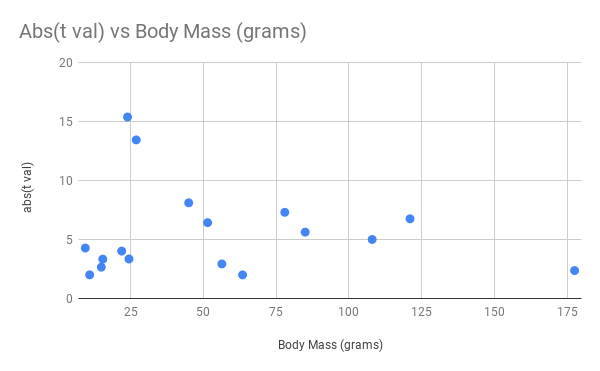
\includegraphics[width=1.0\textwidth]{figures/tValBodyMass.png}
\caption{The plot shows the relationship between the t value magnitudes for the linear-mixed models with temperature anomalies being the independent variable.}
\end{figure}

The first interesting aspect of the scatter plot are the 3 outliers. The smallest, in terms of body mass, of the 3 is the Dark-eyed Junco with a t value magnitude of 15.38 and a body mass of 24 grams. Next is the White-throated sparrow with a t value of 13.44 and mass of 27 grams. Lastly, there is the Northern Cardinal with t value of 8.11 and mass of 45 grams. These three species are especially effected by fluctuations in temperature when it comes to visiting feeders for food.

The second interesting characteristic of the scatter plot, besides the outliers, is that all of the species for this study, regardless of the body mass, were about equally effected by fluctuations in temperatures. This is supported by the fact that the majority of the t values fall within 3 units of 5. A clear example is again the Black-billed Magpie with the body mass of 177.5 grams. It has the t value magnitude of 2.368, which is in the same range as some of the smaller bird species. This is contrary to what we expected for this group of species, as there is no negative relationship.

The last row of Table 4.1 with the Bird Species attribute of All species, presents the summary of the linear-mixed model built with all of the same variables as the previous 23 species. Except there was one key difference, the bird species was also considered a random effect. Recall, that the data source for this was the data frame of all of the individuals bird species' data frames combined. This model allows us to observe the general responses to temperature anomalies across all of the species for the study. 

With this generalized linear model, the slope estimate for all bird species is negative. This is further support for the idea that many of the species visit the bird feeders more often during colder than average days. Additionally, the magnitude of the t value is well above 2, indicating that the effect of temperature anomalies is strong. 

\section{Responses to Wind Speed}

For the analysis with mean wind speed for the day, we expected a species wide decline in abundance at the feeders as the wind speed increased in magnitude. The reason for this is that the conditions for flight are not ideal on windy days. The body mass values of the species are not necessary for this analysis. From the results, there is no evidence of this effect, in fact there is evidence of the opposite effect. When analyzing the bird species individually there appears to be little effect of wind, however with the generalized linear-mixed model for all species there appears to be a positive relationship.

% Please add the following required packages to your document preamble:
% \usepackage{longtable}
% Note: It may be necessary to compile the document several times to get a multi-page table to line up properly
\begin{longtable}[c]{|l|l|l|l|l|}
\caption{Linear-mixed Models: log(Nseen) as a function of the scaled wind speed values.}
\label{my-label}\\
\hline
Bird Species              & Body Mass (grams) & Slope Estimate & t-value & Sig.     \\ \hline
\endhead
%
Brown Creeper             & 7.5               & -0.0042868     & -1.33   & not sig. \\ \hline
Chestnut-backed Chickadee & 9.5               & 0.004216       & 0.548   & not sig. \\ \hline
Mountain Chickadee        & 11                & 1.08E-02       & 1.173   & not sig. \\ \hline
Black-capped Chickadee    & 11.5              & -0.0151193     & -1.393  & not sig. \\ \hline
Chipping Sparrow          & 13.5              & 0.014614       & 1.447   & not sig. \\ \hline
Pine Siskin               & 15                & 2.88E-04       & 0.015   & not sig. \\ \hline
American Goldenfinch      & 15.5              & 0.053091       & 3.959   & sig.     \\ \hline
Common Redpoll            & 15.5              & -0.01463       & -0.872  & not sig. \\ \hline
Tufted Titmouse           & 22                & -5.78E-03      & -0.826  & not sig. \\ \hline
Dark-eyed Junco           & 24                & 0.045943       & 5.581   & sig.     \\ \hline
Downy Woodpecker          & 24.5              & 0.0158335      & 2.527   & sig.     \\ \hline
White-throated Sparrow    & 27                & 5.18E-03       & 0.503   & not sig. \\ \hline
Northern Cardinal         & 45                & 3.33E-02       & 2.29    & sig.     \\ \hline
Northern Mockingbird      & 51.5              & 2.03E-03       & 0.651   & not sig. \\ \hline
Pine Grosbeak             & 56.4              & -1.80E-02      & -0.319  & not sig. \\ \hline
Evening Grosbeak          & 63.5              & 3.69E-02       & 1.296   & not sig. \\ \hline
Hairy Woodpecker          & 67.5              & 1.08E-03       & 0.221   & not sig. \\ \hline
Red-bellied Woodpecker    & 73.5              & 8.49E-03       & 2.028   & sig.     \\ \hline
European Starling         & 78                & 2.68E-02       & 1.856   & not sig. \\ \hline
Blue Jay                  & 85                & -0.014708      & -0.819  & not sig. \\ \hline
Common Grackle            & 108               & 0.03435        & 1.738   & not sig. \\ \hline
Mourning Dove             & 121               & -1.62E-02      & -1.008  & not sig. \\ \hline
Black-billed Magpie       & 177.5             & 0.021912       & 2.007   & sig.     \\ \hline
All species               & NA                & 1.31E-02       & 5.054   & sig.     \\ \hline
\end{longtable}


Table 4.2 presents the slope estimates and t values for the 23 species and the All species linear-mixed model. Many of the models are not significant, with t value magnitudes below 2. However, there is one species with an unusually high absolute t value of 5.581. This species is the Dark-eyed Junco.

It is interesting that the Dark-eyed Junco so far is the only species particularly affected by wind and temperature anomalies. The effect of wind is also interesting as the slope estimate is a positive value. This indicates that as wind speed increased, more individuals were seen at the feeders. This is the opposite of what we were expecting. Perhaps it becomes more difficult to forage for food elsewhere on windy days, making the feeders an easier option. More research is required for this inquiry.

This pattern continues with the All species model. The slope estimate for all of the species is a positive value, moreover the magnitude of the t value is 5.05. This is far above the requirement for significance, indicating the wind speed generally has a strong effect on the species for this study.   

\section{Responses to Precipitation Anomalies}

Our hypothesis for precipitation anomalies was very similar to the wind speed analysis. We expected that as the precipitation levels became higher than average the flight conditions became less ideal, even life threatening. It is possible for birds to suffer torpor and even death when the feathers become too wet~\cite{kennedy1970direct}. This would result in fewer individuals visiting the feeders. The body mass values of the species is not necessary for this analysis. The results, however, did not support our hypothesis.

% Please add the following required packages to your document preamble:
% \usepackage{longtable}
% Note: It may be necessary to compile the document several times to get a multi-page table to line up properly
\begin{longtable}[c]{|l|l|l|l|l|}
\caption{Linear-mixed Models: log(Nseen) as a function of precipitation anomalies.}
\label{my-label}\\
\hline
Bird Species              & Body Mass (grams) & Slope Estimate & t-value  & Sig.     \\ \hline
\endhead
%
Brown Creeper             & 7.5               & 0.0010779      & 0.24     & not sig. \\ \hline
Chestnut-backed Chickadee & 9.5               & 0.007065       & 0.975    & not sig. \\ \hline
Mountain Chickadee        & 11                & 3.59E-02       & 1.548    & not sig. \\ \hline
Black-capped Chickadee    & 11.5              & -0.0001098     & -0.297   & not sig. \\ \hline
Chipping Sparrow          & 13.5              & -0.016613      & -1.394   & not sig. \\ \hline
Pine Siskin               & 15                & 4.89E-02       & 1.253    & not sig. \\ \hline
American Goldenfinch      & 15.5              & 0.034164       & 1.481    & not sig. \\ \hline
Common Redpoll            & 15.5              & 0.035895       & 1.135    & not sig. \\ \hline
Tufted Titmouse           & 22                & -5.01E-03      & -0.576   & not sig. \\ \hline
Dark-eyed Junco           & 24                & 0.050267       & 4.129    & sig.     \\ \hline
Downy Woodpecker          & 24.5              & 0.0108151      & 1.575    & not sig. \\ \hline
White-throated Sparrow    & 27                & 4.32E-03       & 0.667    & not sig. \\ \hline
Northern Cardinal         & 45                & 2.75E-02       & 1.087    & not sig. \\ \hline
Northern Mockingbird      & 51.5              & -2.92E-03      & -1.733   & not sig. \\ \hline
Pine Grosbeak             & 56.4              & -3.84E-02      & -0.256   & not sig. \\ \hline
Evening Grosbeak          & 63.5              & 1.95E-02       & 0.668    & not sig. \\ \hline
Hairy Woodpecker          & 67.5              & 1.91E-02       & 2.032    & sig.     \\ \hline
Red-bellied Woodpecker    & 73.5              & 3.37E-03       & 0.505    & not sig. \\ \hline
European Starling         & 78                & -1.42E-05      & -0.001   & not sig. \\ \hline
Blue Jay                  & 85                & -0.025149      & -0.779   & not sig. \\ \hline
Common Grackle            & 108               & 0.005112       & 0.198    & not sig. \\ \hline
Mourning Dove             & 121               & 3.40E-03       & 0.119    & not sig. \\ \hline
Black-billed Magpie       & 177.5             & 0.03558        & 1.535    & not sig. \\ \hline
All species               & NA                & 1.11E-05       & 2.60E-02 & not sig. \\ \hline
\end{longtable}


Table 4.3 presents the slope estimates and t values for precipitation anomalies as the independent variable. The values are for the 23 species linear-mixed models and the all species general linear-mixed model. One can clearly observe that many of the bird species are not affected by precipitation levels when it came to visiting feeders during the winter. The generalized linear-mixed model is also insignificant. There are even more bird species not significantly effected than with the wind speed analysis. 

The most interesting aspect of these results is once again the Dark-eyed Junco. This species exhibits a positive slope estimate, meaning that as precipitation levels increased, more individuals were spotted at the bird feeders. The t value of 4.129 is also well above 2, indicating the effect of precipitation anomalies is strong. It appears that the Dark-eyed Junco is more sensitive to the climate attributes of temperature variations, wind speed and precipitation variations than the other 22 birds analyzed. Furthermore it is the only species to have significant linear-mixed models with all of 3 independent variables.

\section{Validation}

There are 2 threats to validity given the analysis of the data presented above. The first threat is regarding the generalization of the results to other bird species. In other words, can the insights for the results be applied to other bird species? As mentioned in the earlier section of Bird Species Selection, great care was taken in choosing the appropriate bird species for this project. We worked closely with Professor Francis to select species that are not migratory during winter, with exception of the Evening Grosbeak, allowing us to only study birds that experience winter temperatures. Additionally, a variety of body mass values are represented through the selected species allowing for a wider analysis in regards to the affect of body mass on feeder visits. Lastly, there are total of 23 selected species, which after consultations with Professor Francis was deemed a large enough sample size for this study. This sample size provides an adequate estimate of the non-migratory U.S. winter bird communities in the regions of focus, given the limitations of the Weather Underground API. 

The second threat to validity targets the internal analysis of the responses of the bird species. In other words, is the analysis from the data models of temperature anomalies, wind speed and precipitation anomalies accurate? This threat is disarmed with use of the t values. Only models with t value magnitudes greater than or equal to 2 were considered for analysis, as these models exhibit relationships significant enough to warrant insight. Models not meeting this criteria were ignored, as the insights drawn from them may not be valid. Additionally, in order to use the linear-mixed models certain assumptions must be satisfied. Great care was taken to make sure the assumptions were not violated. These checks were performed through the use of histograms and Q-Q normal plots of the residual values, as previously described in the Assumptions and Residual sections.    





